\section{Derivation of General Formulations}
\label{apx:derivation_of_general_formulations}
The derivations of the starting point formulas presented in Sec.~\ref{sec:methods} are given here.

\subsection{Straight Wire Segment}
The basic geometry of a single wire segment is shown in Fig.~\ref{fig:wire_segment_Hanson_Hirshman_2002_Fig_1}.
\begin{figure}[htbp]
 \centering
 \includegraphics[width=0.5\textwidth]{img/wire_segment_Hanson_Hirshman_2002_Fig_1.png}
 \caption{Geometry of a single wire segment. After Fig.~1 in Ref.~\cite{hanson_hirshman_2002}.}
 \label{fig:wire_segment_Hanson_Hirshman_2002_Fig_1}
\end{figure}
The following geometric quantities with $\mathbf{x}_f \equiv \mathbf{x}_{i+1}$ are defined to ease the rest of the derivation:
\begin{align}
 L                   & \equiv | \mathbf{x}_f - \mathbf{x}_i | \quad , \\
 \hat{\mathbf{e}}    & \equiv \left(\mathbf{x}_f - \mathbf{x}_i\right) / L \quad , \\
 \mathbf{R}_i        & \equiv \mathbf{x} - \mathbf{x}_i \quad , \\
 \mathbf{R}_f        & \equiv \mathbf{x} - \mathbf{x}_f \quad , \\
 R_i                 & \equiv | \mathbf{R}_i | = | \mathbf{x} - \mathbf{x}_i | \quad , \\
 R_f                 & \equiv | \mathbf{R}_f | = | \mathbf{x} - \mathbf{x}_f | \quad , \\
 R_{i ||}            & \equiv \hat{\mathbf{e}} \cdot \mathbf{R}_i \quad , \\
 R_{f ||}            & \equiv \hat{\mathbf{e}} \cdot \mathbf{R}_f \quad , \\
 \mathbf{R}_\perp    & \equiv \mathbf{R}_i - R_{i ||} \hat{\mathbf{e}} \quad , \\
 R_\perp             & \equiv | \mathbf{R}_\perp | \quad \mathrm{and} \\
 \mathbf{c}(\lambda) & \equiv \mathbf{x}_i + \lambda \left(\mathbf{x}_f - \mathbf{x}_i\right) \quad \mathrm{for} \quad 0 \leq \lambda \leq 1 \quad .
\end{align}
The following relations are also needed:
\begin{align}
       L             & = R_{i ||} - R_{f ||} \\
       R_i^2 - R_f^2 & = L \left( R_{i ||} + R_{f ||} \right) \\
\Rightarrow R_{i ||} & = \frac{R_i^2 - R_f^2}{2 L} + \frac{L}{2} \\
\Rightarrow R_{f ||} & = \frac{R_i^2 - R_f^2}{2 L} - \frac{L}{2}
\end{align}

\subsubsection{Magnetic Vector Potential}
The law of Biot and Savart for the magnetic vector potential of a current density distribution $\mathbf{j}(\mathbf{x})$ is as follows~\cite{jackson}:
\begin{equation}
 \mathbf{A}(\mathbf{x}) = \frac{\mu_0}{4 \pi} \int \frac{\mathbf{j}(\mathbf{x}')}{|\mathbf{x} - \mathbf{x}'|} \mathrm{d}\mathbf{x}' \quad .
\end{equation}
The parameterization of points on the line segment $\mathbf{c}(\lambda)$ can be used to apply this to the given geometry of a wire segment:
\begin{align}
 \mathbf{A}(\mathbf{x}) & = \frac{\mu_0 I}{4 \pi} L \hat{\mathbf{e}} \int\limits_0^1 \frac{\mathrm{d}\lambda}{|\mathbf{x} - \mathbf{c}(\lambda)|} \\
        ~               & = \frac{\mu_0 I}{4 \pi} L \hat{\mathbf{e}} \int\limits_0^1 \frac{\mathrm{d}\lambda}{|\mathbf{x} - \mathbf{x}_i - \lambda L \hat{\mathbf{e}}|} \quad .
\end{align}
A little bit of geometric intuition is needed to simplify the denominator of the integral:
\begin{align}
 \mathbf{x} - \mathbf{x}_i - \lambda L \hat{\mathbf{e}}
   & = \mathbf{R}_i - \lambda L \hat{\mathbf{e}} \\
 ~ & = \mathbf{R}_i - R_{i ||} \hat{\mathbf{e}} + R_{i ||} \hat{\mathbf{e}} - \lambda L \hat{\mathbf{e}} \\
 ~ & = \mathbf{R}_i - R_{i ||} \hat{\mathbf{e}} + \left( R_{i ||} - \lambda L \right) \hat{\mathbf{e}} \\
 ~ & = \mathbf{R}_\perp + \left( R_{i ||} - \lambda L \right) \hat{\mathbf{e}} \quad .
\end{align}
Note that, in particular, $\mathbf{R}_\perp \perp \hat{\mathbf{e}}$ and thus (since $|\hat{\mathbf{e}}|$ = 1) due to Pythagoras:
\begin{equation}
 | \mathbf{x} - \mathbf{x}_i - \lambda L \hat{\mathbf{e}} |^2 = R_\perp^2 + \left( R_{i ||} - \lambda L \right)^2
\end{equation}
and finally with $R_\perp^2 = R_i^2 - R_{i ||}^2$ (also due to Pythagoras):
\begin{align}
 | \mathbf{x} - \mathbf{x}_i - \lambda L \hat{\mathbf{e}} |^2
   & = R_i^2 - R_{i ||}^2 + R_{i ||}^2 - 2 \lambda L R_{i ||} + \lambda^2 L^2 \\
 ~ & = R_i^2 - 2 \lambda L R_{i ||} + \lambda^2 L^2 \quad .
\end{align}
It follows:
\begin{equation}
 \mathbf{A}(\mathbf{x})
 = \frac{\mu_0 I}{4 \pi} L \hat{\mathbf{e}} \int\limits_0^1 \frac{\mathrm{d}\lambda}{\sqrt{R_i^2 - 2 \lambda L R_{i ||} + \lambda^2 L^2}} \quad . \label{eqn:A_integral}
\end{equation}
For $X = a x^2 + b x + c$ with $a>0$ the following relation holds~\cite{bronstein}:
\begin{equation}
 \int \frac{\mathrm{d}x}{\sqrt{X}} = \frac{1}{\sqrt{a}} \log \left( 2 \sqrt{a X} + 2 a x + b \right) \quad .
\end{equation}
Here, $x = \lambda$, $a = L^2$, $b=-2 L R_{i ||}$ and $c=R_i^2$.
The corresponding antiderivative of the integrand in \eqn{eqn:A_integral} is:
\begin{equation}
   \int\frac{\mathrm{d}\lambda}{\sqrt{R_i^2 - 2 \lambda L R_{i ||} + \lambda^2 L^2}}
 = \frac{1}{L} \log \left( 2 \sqrt{L^2\left( L^2 \lambda^2 - 2 L R_{i ||} \lambda + R_i^2 \right)} + 2 L^2 \lambda - 2 L R_{i ||} \right) \quad .
\end{equation}
The definite integral in \eqn{eqn:A_integral} is therefore solved by the following expression:
\begin{align}
 ~ & \int\limits_0^1 \frac{\mathrm{d}\lambda}{\sqrt{R_i^2 - 2 \lambda L R_{i ||} + \lambda^2 L^2}} \\
 = & \frac{1}{L} \left[ \log \left( 2 \sqrt{L^2\left( L^2 - 2 L R_{i ||} + R_i^2 \right)} + 2 L^2 - 2 L R_{i ||} \right) - \log \left( 2 \sqrt{L^2 R_i^2 } - 2 L R_{i ||} \right) \right] \\
 = & \frac{1}{L} \log \left( \frac{ \bcancel{2 L} \sqrt{L^2 - 2 L R_{i ||} + R_i^2} + \bcancel{2} L^{\bcancel{2}} - \bcancel{2 L} R_{i ||} }{ \bcancel{2 L} R_i - \bcancel{2 L} R_{i ||} } \right)
\end{align}
Note that
\begin{align}
                             L^2 & = L (R_{i ||} - R_{f ||} ) \\
                              ~  & = L R_{i ||} - L R_{f ||} \\
\Rightarrow -2 L R_{i ||} + L^2  & = - \bcancel{2} L R_{i ||}  + \bcancel{L R_{i ||}} - L R_{f ||} \\
                              ~  & = -L (R_{i ||} + R_{f ||} ) \\
                              ~  & = R_f^2 - R_i^2 \\
\Rightarrow                R_f^2 & = R_i^2 -2 L R_{i ||} + L^2 \quad .
\end{align}
Therefore:
\begin{equation}
 \int\limits_0^1 \frac{\mathrm{d}\lambda}{\sqrt{R_i^2 - 2 \lambda L R_{i ||} + \lambda^2 L^2}}
 = \frac{1}{L} \log \left( \frac{ R_f - R_{f ||} }{ R_i - R_{i  \,\mathrm{d}\varphi||} } \right) \quad .
\end{equation}
Inserting this into \eqn{eqn:A_integral} leads to the first intermediate result:
\begin{equation}
   \mathbf{A}(\mathbf{x})
 = \frac{\mu_0 I}{4 \pi} \bcancel{L} \bcancel{\frac{1}{L}} \log \left( \frac{ R_f - R_{f ||} }{ R_i - R_{i ||} } \right) \hat{\mathbf{e}}
 = \frac{\mu_0 I}{4 \pi}                                   \log \left( \frac{ R_f - R_{f ||} }{ R_i - R_{i ||} } \right) \hat{\mathbf{e}} \quad . \label{eqn:A_first}
\end{equation}
However, if the point $\mathbf{x}$ is located on the line extension of the wire segment, $R_i = R_{i ||}$ and $R_f = R_{f ||}$,
which leads to a $0/0$ division if this formula is directly evaluated.
The solution is to cancel the singular term $(L + R_f - R_i)$, which is also zero for points on the line extension of the wire segment,
in the numerator and the denominator of \eqn{eqn:A_first}.
A second look resolves this:
\begin{align}
\frac{ R_f - R_{f ||} }{ R_i - R_{i ||} }
 = & \frac{ 2 L \left( R_f - R_{f ||} \right) }{ 2 L \left( R_i - R_{i ||} \right) }
 =   \frac{ 2 L R_f - 2 L \left( \frac{R_i^2 - R_f^2}{2 L} - \frac{L}{2} \right) }{ 2 L R_i - 2 L \left( \frac{R_i^2 - R_f^2}{2 L} + \frac{L}{2} \right) } \\
 = & \frac{ 2 L R_f - R_i^2 + R_f^2 + L^2 }{ 2 L R_i - R_i^2 + R_f^2 - L^2 } \\
 = & \frac{ 2 L R_f - R_i^2 + R_f^2 + L^2 + L R_i - L R_i + R_i R_f - R_i R_f}{ 2 L R_i - R_i^2 + R_f^2 - L^2 + L R_f - L R_f + R_i R_f - R_i R_f } \\
 = & \frac{\bcancel{(L + R_f - R_i)}(R_f + R_i + L)}{\bcancel{(L + R_f - R_i)}(R_f + R_i - L)}
 =   \frac{R_f + R_i + L}{R_f + R_i - L} \quad .
\end{align}
It follows for the vector potential expression:
\begin{equation}
 \mathbf{A}(\mathbf{x}) = \frac{\mu_0 I}{4 \pi} \log \left( \frac{R_f + R_i + L}{R_f + R_i - L} \right) \hat{\mathbf{e}} \quad . \label{eqn:A_second}
\end{equation}
The authors of Ref.~\cite{hanson_hirshman_2002} suggest to normalize the length of the wire segment:
\begin{equation}
 \frac{R_f + R_i + L}{R_f + R_i - L} = \frac{1 + \epsilon}{1 - \epsilon} \quad \mathrm{with} ~ \epsilon \equiv \frac{L}{R_i + R_f} \quad ,
\end{equation}
leading to
\begin{equation}
 \mathbf{A}(\mathbf{x}) = \frac{\mu_0 I}{4 \pi} \log\left(\frac{1 + \epsilon}{1 - \epsilon} \right) \hat{\mathbf{e}} \quad . \label{eqn:A_log_eps}
\end{equation}
This is the result for the magnetic vector potential of a filamentary wire segment presented in Ref.~\cite{hanson_hirshman_2002}.
However, for $\epsilon \rightarrow 0$, the numerical evaluation of this expression is problematic.
It is therefore suggested to use the following expression, which works for points extremely close to,
extremely far away from and all in-between locations with respect to the wire segment.
Note that
\begin{equation}
 \mathrm{artanh}\left( \epsilon \right) = \frac{1}{2} \log\left(\frac{1 + \epsilon}{1 - \epsilon} \right) \quad ,
\end{equation}
leading to
\begin{equation}
 \boxed{\mathbf{A}(\mathbf{x}) = \frac{\mu_0 I}{2 \pi} \, \mathrm{artanh} \left( \epsilon \right) \hat{\mathbf{e}}} \quad . \label{eqn:A_artanh}
\end{equation}

\subsubsection{Magnetic Field}
The magnetic field $\mathbf{B}(\mathbf{x})$ is computed from $\mathbf{B} = \nabla \times \mathbf{A}$, applied to \eqn{eqn:A_log_eps}.
Define
\begin{equation}
 f(\epsilon) \equiv \log\left(\frac{1 + \epsilon}{1 - \epsilon} \right)
\end{equation}
and it follows:
\begin{equation}
  \frac{4 \pi}{\mu_0 I} \mathbf{B}
 = \nabla \times \left( f(\epsilon) \hat{\mathbf{e}} \right)
 = \nabla f(\epsilon) \times \hat{\mathbf{e}} + f(\epsilon) \underbrace{\nabla \times \hat{\mathbf{e}}}_{=0}
 = f'(\epsilon) \nabla \epsilon \times \hat{\mathbf{e}} \quad .
\end{equation}
Note that
\begin{equation}
   \nabla \epsilon
 = \nabla \left( \frac{L}{R_i + R_f} \right)
 = \frac{-L}{(R_i + R_f)^2}\left( \nabla R_i + \nabla R_f \right)
 = \frac{-L}{(R_i + R_f)^2}\left( \frac{\mathbf{R}_i}{R_i} + \frac{\mathbf{R}_f}{R_f} \right) \quad .
\end{equation}
It follows:
\begin{align}
   \frac{4 \pi}{\mu_0 I} \mathbf{B}
 = & f'(\epsilon) \frac{-L}{(R_i + R_f)^2} \left( \frac{\mathbf{R}_i}{R_i} + \frac{\mathbf{R}_f}{R_f} \right) \times \hat{\mathbf{e}} \\
 = & f'(\epsilon) \frac{L}{(R_i + R_f)^2} \, \hat{\mathbf{e}} \times \left( \frac{\mathbf{R}_i}{R_i} + \frac{\mathbf{R}_f}{R_f} \right) \\
 = & f'(\epsilon) \frac{\epsilon^2}{L}    \, \hat{\mathbf{e}} \times \left( \frac{\mathbf{R}_i}{R_i} + \frac{\mathbf{R}_f}{R_f} \right) \quad . \label{eqn:B_intermediate}
\end{align}
Also:
\begin{align}
   \frac{\mathbf{R}_i}{R_i} + \frac{\mathbf{R}_f}{R_f}
 = & \frac{\mathbf{R}_i}{R_i} + \frac{\mathbf{R}_i - L \hat{\mathbf{e}} }{R_f}
 =   \frac{R_f \mathbf{R}_i + R_i (\mathbf{R}_i - L \hat{\mathbf{e}}) }{R_i R_f}
 =   \frac{(R_f+R_i) \mathbf{R}_i + R_i L \hat{\mathbf{e}} }{R_i R_f} \\
 = & \frac{R_f+R_i}{R_i R_f} \mathbf{R}_i + \frac{R_i L}{R_i R_f} \, \hat{\mathbf{e}}
\end{align}
and therefore:
\begin{equation}
   \hat{\mathbf{e}} \times \left( \frac{\mathbf{R}_i}{R_i} + \frac{\mathbf{R}_f}{R_f} \right)
 = \hat{\mathbf{e}} \times \left( \frac{R_f+R_i}{R_i R_f} \mathbf{R}_i + \frac{R_i L}{R_i R_f} \, \hat{\mathbf{e}} \right)
 = \frac{R_f+R_i}{R_i R_f} \, \hat{\mathbf{e}} \times \mathbf{R}_i \quad ,
\end{equation}
since $\hat{\mathbf{e}} \times \hat{\mathbf{e}} = 0$.
Inserting this into \eqn{eqn:B_intermediate} leads to:
\begin{equation}
   \frac{4 \pi}{\mu_0 I} \mathbf{B}
 = f'(\epsilon) \frac{\epsilon^{\bcancel{2}}}{\bcancel{L}} \, \frac{\bcancel{R_f+R_i}}{R_i R_f} \, \hat{\mathbf{e}} \times \mathbf{R}_i
 = f'(\epsilon) \frac{\epsilon}{R_i R_f} \, \hat{\mathbf{e}} \times \mathbf{R}_i \label{eqn:B_intermediate_2}
\end{equation}
Next, look at $f'(\epsilon)$:
\begin{equation}
   f'(\epsilon)
 = \frac{\bcancel{1 - \epsilon}}{1 + \epsilon} \cdot \frac{1 (1-\epsilon) - (1+\epsilon) (-1)}{(1 - \epsilon)^{\bcancel{2}}}
 = \frac{1 - \epsilon + 1 + \epsilon}{(1 + \epsilon)(1 - \epsilon)}
 = \frac{2}{1 - \epsilon^2}
\end{equation}
and insert this into \eqn{eqn:B_intermediate_2}:
\begin{align}
   \frac{4 \pi}{\mu_0 I} \mathbf{B}
 = & \frac{2 \epsilon}{1 - \epsilon^2} \cdot \frac{1}{R_i R_f} \, \hat{\mathbf{e}} \times \mathbf{R}_i \\
 = & \frac{2 L}{\bcancel{R_i + R_f}} \cdot \frac{(R_i + R_f)^{\bcancel{2}}}{(R_i + R_f)^2 - L^2} \cdot \frac{1}{R_i R_f} \, \hat{\mathbf{e}} \times \mathbf{R}_i \quad .
\end{align}
This results in the final expression for the magnetic field:
\begin{equation}
 \boxed{\mathbf{B} (\mathbf{x}) = \frac{\mu_0 I}{4 \pi} \frac{2 L (R_i + R_f)}{R_i R_f} \frac{1}{(R_i + R_f)^2 - L^2} \, \hat{\mathbf{e}} \times \mathbf{R}_i } \quad .
\end{equation}

\subsection{Circular Wire Loop}
The basic geometry of a circular wire loop under consideration here is shown in Fig.~\ref{fig:circularWireLoop}.
\begin{figure}[htbp]
 \centering
 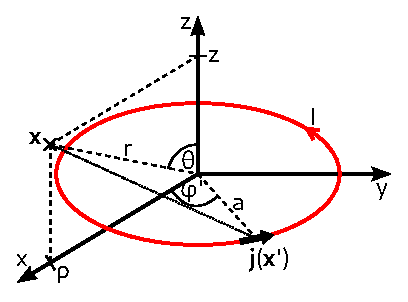
\includegraphics[width=0.5\textwidth]{img/circularWireLoop.eps}
 \caption{Geometry of a circular wire loop centered at the origin with normal vector aligned with the $z$-axis.
          The radius of the loop is denoted $a$ and a current $I$ flows in the indicated direction.
          The magnetic field and vector potential are to be evaluated at the point $\mathbf{x}$ in the ($x$, $z$)-plane.}
 \label{fig:circularWireLoop}
\end{figure}

The current density of the wire loop can be expressed as follows:
\begin{equation}
  \mathbf{j}(\mathbf{x}') = I \delta(\rho' - a) \delta(z') \,\hat{\mathbf{e}}_{\varphi'} \, .
\end{equation}

\subsubsection{Magnetic Vector Potential}
The Biot-Savart law for the magnetic vector potential reads:
\begin{align}
  \mathbf{A}(\mathbf{x}) &= \frac{\mu_0  }{4 \pi}
                            \int_{\realnumbers^3}
                              \frac{\mathbf{j}(\mathbf{x}')}{|\mathbf{x} - \mathbf{x}'|} \,\mathrm{d}^3\mathbf{x}' \nonumber \\
             ~           &= \frac{\mu_0 I}{4 \pi}
                            \int_{\realnumbers^3}
                              \frac{\delta(\rho' - a) \delta(z')}{|\mathbf{x} - \mathbf{x}'|} \,\hat{\mathbf{e}}_{\varphi'}
                              \,\mathrm{d}^3\mathbf{x}' \nonumber \\
             ~           &= \frac{\mu_0 I}{4 \pi}
                            \int\limits_{-\infty}^{\infty} \int\limits_{0}^{2 \pi} \int\limits_{0}^{\infty}
                              \frac{\delta(\rho' - a) \delta(z')}{|\mathbf{x} - \mathbf{x}'|} \,\hat{\mathbf{e}}_{\varphi'}
                              \rho' \,\mathrm{d} \rho' \,\mathrm{d} \varphi'  \,\mathrm{d} z' \label{eqn:vecpot_loop_general}
\end{align}
where a change of variables from cartesian coordinates to cylindrical coordinates was performed in the integral.
The differential volume element was adjusted according to
$\,\mathrm{d}^3\mathbf{x}' = \rho' \,\mathrm{d} \rho' \,\mathrm{d} \varphi'  \,\mathrm{d} z'$.
The coordinate system is rotated around the $z$ axis to yield $\varphi=0$ for the evaluation location $\mathbf{x}$
which is generally acceptable due to the rotational symmetry of the circular wire loop.
Then, $\mathbf{x} = (x, y, z)$ in cartesian coordinates with
\begin{align}
  x &= \rho \cos(\varphi) = \rho \\
  y &= \rho \sin(\varphi) = 0    \, .
\end{align}
The distance $|\mathbf{x} - \mathbf{x}'|$ is then:
\begin{align}
  |\mathbf{x} - \mathbf{x}'| &= \sqrt{(\rho - \rho' \cos(\varphi'))^2 + \rho'^2 \sin^2(\varphi') + (z - z')^2} \nonumber \\
              ~              &= \sqrt{ \rho^2 + \rho'^2 (\cos(\varphi'))^2 + \sin^2(\varphi')) - 2 \rho \rho' \cos(\varphi') + (z - z')^2} \nonumber \\
              ~              &= \sqrt{ \rho^2 + \rho'^2 + (z - z')^2 - 2 \rho \rho' \cos(\varphi')} \, .
\end{align}
Inserting this into \eqn{eqn:vecpot_loop_general} leads to:
\begin{equation}
  \mathbf{A}(\mathbf{x}) = \frac{\mu_0 I}{4 \pi} \int\limits_{-\infty}^{\infty} \int\limits_{0}^{2 \pi} \int\limits_{0}^{\infty}
                                                             \frac{\delta(\rho' - a) \delta(z')}{\sqrt{ \rho^2 + \rho'^2 + (z - z')^2 - 2 \rho \rho' \cos(\varphi')}}
                                                             \,\hat{\mathbf{e}}_{\varphi'}
                                                             \rho' \,\mathrm{d} \rho' \,\mathrm{d} \varphi'  \,\mathrm{d} z'
\end{equation}
and the integrals over $\rho'$ and $z'$ can be evaluated already:
\begin{equation}
  \mathbf{A}(\mathbf{x}) = \frac{\mu_0 I a}{4 \pi}
                           \int\limits_{0}^{2 \pi}
                             \frac{\hat{\mathbf{e}}_{\varphi'} \,\mathrm{d} \varphi'}{\sqrt{ \rho^2 + a^2 + z^2 - 2 \rho a \cos(\varphi')}} \, . \label{eqn:vecpot_loop_phiprime}
\end{equation}
The cylindrical components of the magnetic vector potential~$\mathbf{A}$ are obtained
by dotting above result with the cylindrical unit vector at the evaluation location~$\mathbf{x}$:
\begin{equation}
  \mathbf{A}(\mathbf{x}) =   A_\rho    \,\hat{\mathbf{e}}_\rho
                           + A_\varphi \,\hat{\mathbf{e}}_\varphi
                           + A_z       \,\hat{\mathbf{e}}_z
\end{equation}
with
\begin{align}
  A_\rho    &= \mathbf{A}(\mathbf{x}) \cdot \,\hat{\mathbf{e}}_\rho    \\
  A_\varphi &= \mathbf{A}(\mathbf{x}) \cdot \,\hat{\mathbf{e}}_\varphi \\
  A_z       &= \mathbf{A}(\mathbf{x}) \cdot \,\hat{\mathbf{e}}_z       \, .
\end{align}
The dot products of the cylindrical unit vectors are:
\begin{align}
  \hat{\mathbf{e}}_{\varphi'} \cdot \,\hat{\mathbf{e}}_\rho    &= \begin{pmatrix} -\sin(\varphi') \\ \cos(\varphi') \\ 0 \end{pmatrix}
                                                                  \cdot
                                                                  \begin{pmatrix}  \cos(\varphi ) \\ \sin(\varphi ) \\ 0 \end{pmatrix}
                                                                = \begin{pmatrix} -\sin(\varphi') \\ \cos(\varphi') \\ 0 \end{pmatrix}
                                                                  \cdot
                                                                  \begin{pmatrix}  1 \\ 0 \\ 0 \end{pmatrix}
                                                                = -\sin(\varphi') \\
  \hat{\mathbf{e}}_{\varphi'} \cdot \,\hat{\mathbf{e}}_\varphi &= \begin{pmatrix} -\sin(\varphi') \\ \cos(\varphi') \\ 0 \end{pmatrix}
                                                                  \cdot
                                                                  \begin{pmatrix} -\sin(\varphi ) \\ \cos(\varphi ) \\ 0 \end{pmatrix}
                                                                = \begin{pmatrix} -\sin(\varphi') \\ \cos(\varphi') \\ 0 \end{pmatrix}
                                                                  \cdot
                                                                  \begin{pmatrix}  0 \\ 1 \\ 0 \end{pmatrix}
                                                                =  \cos(\varphi') \\
  \hat{\mathbf{e}}_{\varphi'} \cdot \,\hat{\mathbf{e}}_z       &= \begin{pmatrix} -\sin(\varphi') \\ \cos(\varphi') \\ 0 \end{pmatrix}
                                                                  \cdot
                                                                  \begin{pmatrix} 0 \\ 0 \\ 1 \end{pmatrix}
                                                                = 0 \, . \label{eqn:e_phiprime_dot_ez}
\end{align}
The expression from \eqn{eqn:vecpot_loop_phiprime} is inserted into above expressions.
The vertical component~$A_z$ vanishes trivially since the unit vectors are orthogonal,
as can be seen from \eqn{eqn:e_phiprime_dot_ez}.
For the radial component $A_\rho$ it follows:
\begin{equation}
  A_\rho = \frac{\mu_0 I a}{4 \pi}
           \int\limits_{0}^{2 \pi}
             \frac{-\sin(\varphi') \,\mathrm{d} \varphi'}{\sqrt{ \rho^2 + a^2 + z^2 - 2 \rho a \cos(\varphi')}} = 0 \, ,
\end{equation}
since the integrand is an odd function of $\varphi'$.
The tangential component $A_\varphi$ is non-zero because the integrand is an even function of $\varphi'$.
It is given by:
\begin{equation}
  A_\varphi(\rho, z) = \frac{\mu_0 I a}{4 \pi}
                       \int\limits_{0}^{2 \pi}
                         \frac{\cos(\varphi') \,\mathrm{d} \varphi'}{\sqrt{ \rho^2 + a^2 + z^2 - 2 \rho a \cos(\varphi')}} \, , \label{eqn:a_phi_general}
\end{equation}
leading to
\begin{equation}
  \mathbf{A}(\mathbf{x}) = A_\varphi(\rho, z) \,\hat{\mathbf{e}}_\varphi \, . \label{eqn:a_cwl_components}
\end{equation}
A change of variables from $\varphi'$ to $\beta$ is performed in order to solve \eqn{eqn:a_phi_general}:
\begin{equation}
 \varphi' = 2 \beta + \pi
\end{equation}
which implies
\begin{align}
 \frac{\mathrm{d}\varphi'}{\mathrm{d}\beta} = 2     &\Rightarrow \mathrm{d}\varphi' = 2 \mathrm{d}\beta \\
                                 \varphi'_0 = 0     &\Rightarrow           \beta_0 = - \frac{\pi}{2}   \\
                                 \varphi'_1 = 2 \pi &\Rightarrow           \beta_1 =   \frac{\pi}{2}   \, .
\end{align}
It follows for \eqn{eqn:a_phi_general}:
\begin{equation}
 A_\varphi(\rho, z) = \frac{\mu_0 I a}{4 \pi}
                       \int\limits_{-\pi/2}^{\pi/2}
                         \frac{2 \cos(2 \beta + \pi) \,\mathrm{d}\beta}
                              {\sqrt{\rho^2 + a^2 + z^2 - 2 \rho a \cos(2 \beta + \pi)}} \, .
\end{equation}
Note that $\cos(2 \beta + \pi) = - \cos(2 \beta)$:
\begin{equation}
 A_\varphi(\rho, z) = \frac{\mu_0 I a}{2 \pi}
                       \int\limits_{-\pi/2}^{\pi/2}
                         \frac{-\cos(2 \beta) \,\mathrm{d}\beta}
                              {\sqrt{\rho^2 + a^2 + z^2 + 2 \rho a \cos(2 \beta)}} \, . \label{eqn:a_phi_progress}
\end{equation}
In the numerator of the integrand it follows:
\begin{equation}
 -\cos(2 \beta) = -\left(\cos^2(\beta) - \sin^2(\beta) \right) = \sin^2(\beta) - \cos^2(\beta) \, .
\end{equation}
The denominator of the integrand can be reformulated by introducing normalized coordinates
$\rho' = \rho/a$ and $z' = z/a$ as follows:
\begin{align}
 ~ & \rho^2 + a^2 + z^2 + 2 \rho a \cos(2 \beta) \nonumber \\
 ~ &= a^2 \left[z'^2 +      \rho'^2 + 1        + 2 \rho' \cos(2 \beta)         \right] \nonumber \\
 ~ &= a^2 \left[z'^2 + (1 + \rho')^2 - 2 \rho' + 2 \rho' \cos(2 \beta)         \right] \nonumber \\
 ~ &= a^2 \left[z'^2 + (1 + \rho')^2 - 2 \rho' \left(1 - \cos(2 \beta) \right) \right] \nonumber \\
 ~ &= a^2 \left[z'^2 + (1 + \rho')^2 - 2 \rho' \left(1 + \sin^2(\beta) - \cos^2(\beta) \right) \right] \nonumber \\
 ~ &= a^2 \left[z'^2 + (1 + \rho')^2 - 2 \rho' \left(\bcancel{\cos^2(\beta)} + \sin^2(\beta) + \sin^2(\beta) \bcancel{- \cos^2(\beta)} \right) \right] \nonumber \\
 ~ &= a^2 \left[z'^2 + (1 + \rho')^2 - 4 \rho' \sin^2(\beta) \right] \nonumber \\
 ~ &= a^2 \left( z'^2 + (1 + \rho')^2 \right) \Biggl[1 - \underbrace{\frac{4 \rho'}{z'^2 + (1 + \rho')^2}}_{\equiv k^2} \sin^2(\beta) \Biggr] \nonumber \\
 ~ &= a^2 \left( z'^2 + (1 + \rho')^2 \right) \left [1 - k^2 \sin^2(\beta) \right] \label{eqn:a_phi_denom_refactor_start}
\end{align}
with
\begin{equation}
 k^2 = \frac{4 \rho'}{z'^2 + (1 + \rho')^2} \, . \label{eqn:my_k_sq}
\end{equation}
Inserting this into \eqn{eqn:a_phi_progress} leads to:
\begin{equation}
 A_\varphi(\rho', z') = \frac{\mu_0 I}
                           {2 \pi}
                      \frac{1}
                           {\sqrt{z'^2 + (1 + \rho')^2}}
                      \int\limits_{-\pi/2}^{\pi/2}
                        \frac{\sin^2(\beta) - \cos^2(\beta)}
                             {\sqrt{1 - k^2 \sin^2(\beta)}}
                        \,\mathrm{d}\beta \, .
\end{equation}
Focusing again on the denominator of the integrand:
\begin{align}
 1 - k^2 \sin^2(\beta)
   &= \cos^2(\beta) + \sin^2(\beta) - \frac{4 \rho'}{z'^2 + (1 + \rho')^2} \sin^2(\beta) \nonumber \\
 ~ &= \cos^2(\beta) + \left(1 - \frac{4 \rho'}{z'^2 + (1 + \rho')^2}\right) \sin^2(\beta) \nonumber \\
 ~ &= \cos^2(\beta) + \frac{z'^2 + (1 + \rho')^2 - 4 \rho'}{z'^2 + (1 + \rho')^2} \sin^2(\beta) \nonumber \\
 ~ &= \cos^2(\beta) + \underbrace{\frac{z'^2 + (1 - \rho')^2}{z'^2 + (1 + \rho')^2}}_{\equiv k_c^2} \sin^2(\beta) \nonumber \\
 ~ &= \cos^2(\beta) + k_c^2 \sin^2(\beta) \label{eqn:a_phi_denom_refactor_done}
\end{align}
with
\begin{equation}
 k_c^2 = \frac{z'^2 + (1 - \rho')^2}{z'^2 + (1 + \rho')^2} \, , \label{eqn:k_c_final}
\end{equation}
leading to:
\begin{equation}
 A_\varphi(\rho', z') = \frac{\mu_0 I}
                           {2 \pi}
                      \frac{1}
                           {\sqrt{z'^2 + (1 + \rho')^2}}
                      \int\limits_{-\pi/2}^{\pi/2}
                        \frac{\sin^2(\beta) - \cos^2(\beta)}
                             {\sqrt{\cos^2(\beta) + k_c^2 \sin^2(\beta)}}
                        \,\mathrm{d}\beta \, .
\end{equation}
The integrand is symmetric about $0$ and therefore the integration domain can be halved if a factor of $2$ is included:
\begin{equation}
 A_\varphi(\rho', z') = \frac{\mu_0 I}
                           {\pi}
                      \frac{1}
                           {\sqrt{z'^2 + (1 + \rho')^2}}
                      \int\limits_{0}^{\pi/2}
                        \frac{\sin^2(\beta) - \cos^2(\beta)}
                             {\sqrt{\cos^2(\beta) + k_c^2 \sin^2(\beta)}}
                        \,\mathrm{d}\beta \, .
\end{equation}
The remaining integral is a complete elliptic integral which can be expressed using the form
introduced by Bulirsch~\cite{bulirsch_3}:
\begin{equation}
  \mathrm{cel}(k_c, p, a, b)
= \int\limits_{0}^{\pi/2}
   \frac{a \cos^2(\varphi) + b \sin^2(\varphi)}
        {  \cos^2(\varphi) + p \sin^2(\varphi)}
   \frac{\mathrm{d}\varphi}
        {\sqrt{\cos^2(\varphi) + k_\mathrm{c}^2 \sin^2(\varphi)}} \, .
\end{equation}
Note that the parameter $a$ of $\mathrm{cel}(k_c, p, a, b)$ is not to be confused with the radius of the wire loop.
A numerical implementation of the general complete elliptic integral $\mathrm{cel}(k_c, p, a, b)$ is provided in the cited article.
The use of this particular implementation is inspired by Ref.~\cite{teal}.
Putting above results together, we arrive at the following expression for $A_\varphi$:
\begin{equation}
 \boxed{A_\varphi(\rho', z') = \frac{\mu_0 I}{\pi}
                               \frac{1}{\sqrt{z'^2 + (1 + \rho')^2}}
                               \,\mathrm{cel}(k_c, 1, -1, 1)} \, . \label{eqn:A_phi_final}
\end{equation}
In Eqn.~(5.37) of Ref.~\cite{jackson} the tangential component is given by:
\begin{align}
  A_\varphi(r, \theta) &= \frac{\mu_0}{4 \pi}
                          \frac{4 I a}{\sqrt{a^2 + r^2 + 2 a r \sin(\theta)}}
                          \left[
                            \frac{(2 - k^2)K(k) - 2 E(k)}{k^2}
                          \right] \label{eqn:aphi_initial}
\end{align}
with
\begin{equation}
  k^2 = \frac{4 a r \sin(\theta)}{a^2 + r^2 + 2 a r \sin(\theta)} \, .
\end{equation}
Here, $K(k)$ and $E(k)$ are the complete elliptic integrals of the first and second kind, respectively.
Spherical coordinates are used with $r \sin(\theta) = \rho$ and $r^2 = \rho^2 + z^2$.
In order to bring this to the form in \eqn{eqn:A_phi_final},
an expression for the linear combination of $K(k)$ and $E(k)$ from Ref.~\cite{bulirsch_3} is used:
\begin{equation}
  \lambda K(k) + \mu E(k) = \,\mathrm{cel}(k_c, 1, \lambda + \mu, \lambda + \mu k_c^2)
\end{equation}
where
\begin{equation}
  k^2 + k_\mathrm{c}^2 = 1 \, .
\end{equation}
The argument of the elliptic integrals is considered first:
\begin{align}
  k^2 &= \frac{4 a r \sin(\theta)}{a^2 + r^2 + 2 a r \sin(\theta)}
       = \frac{4 a \rho}{a^2 + r^2 + 2 a \rho}
       = \frac{4 \bcancel{a} \rho}{a^{\bcancel{2}} \left(1 + \frac{r^2}{a^2} + 2 \frac{\rho}{a} \right)} \nonumber \\
  ~   &= \frac{4 \rho'}{1 + \frac{r^2}{a^2} + 2 \rho'}
       = 4 \rho' \left( 1 + \frac{\rho^2 + z^2}{a^2} + 2 \rho' \right)^{-1}
       = 4 \rho' \left( 1 + \rho'^{2} + z'^{2} + 2 \rho' \right)^{-1} \nonumber \\
  ~   &= \frac{4 \rho'}{z'^2 + (1 + \rho')^2} \, .
\end{align}
Thus, $k^2$ from Ref.~\cite{jackson} is equivalent to $k^2$ in \eqn{eqn:my_k_sq}.
Inserting this into \eqn{eqn:aphi_initial} leads to:
\begin{align}
  A_\varphi(r, \theta) &= \frac{\mu_0 I}{\bcancel{2} \pi}
                          \frac{\bcancel{2}}{\sqrt{z'^2 + (1 + \rho')^2}}
                          \left[
                            \frac{(2 - k^2)K(k) - 2 E(k)}{k^2}
                          \right] \nonumber \\
           ~           &= \frac{\mu_0 I}{\pi}
                          \frac{1}{\sqrt{z'^2 + (1 + \rho')^2}}
                          \left[
                            \frac{(2 - k^2)K(k) - 2 E(k)}{k^2}
                          \right] \, .
\end{align}
The coefficients of the elliptic integrals are given as follows:
\begin{align}
  \lambda &= \frac{2 - k^2}{k^2} = \frac{2}{k^2} - 1 \\
  \mu     &= -\frac{2}{k^2}
\end{align}
and their combinations are as follows:
\begin{align}
  \lambda + \mu       &= \frac{2}{k^2} - 1 - \frac{2}{k^2}     = -1 \\
  \lambda + \mu k_c^2 &= \frac{2}{k^2} - 1 - \frac{2}{k^2} (1 - k^2) \nonumber \\
          ~           &= \frac{2}{k^2} - 1 - \frac{2}{k^2} + 2 =  1 \, .
\end{align}
Putting above results together, we arrive at the following expression for $A_\varphi$:
\begin{equation}
 \boxed{A_\varphi(r, \theta) = \frac{\mu_0 I}{\pi}
                            \frac{1}{\sqrt{z'^2 + (1 + \rho')^2}} \,\mathrm{cel}(k_c, 1, -1, 1)}
\end{equation}
with $\rho' = r/a \sin(\theta)$, $z' = \sqrt{r^2 - \rho^2}/a$ and $k_c$ given by \eqn{eqn:k_c_final}).
It is favourable for numerical evaluation of $A_\varphi$ to use the form given in \eqn{eqn:A_phi_final}
where the linear combination of the complete elliptic integrals is embedded in the parameters of $\mathrm{cel}(k_c, p, a, b)$
and no precautions need to be taken to deal with cancellations in \eqn{eqn:aphi_initial}.

\subsubsection{Magnetic Field}
The magnetic field is computed using $\mathbf{B} = \nabla \times \mathbf{A}$.
In cylindrical coordinates with the form of the magnetic vector potential from \eqn{eqn:a_cwl_components}
the curl is given as follows:
\begin{equation}
  \mathbf{B}(\mathbf{x})
= B_\rho \hat{\mathbf{e}}_\rho + B_z \hat{\mathbf{e}}_z
\end{equation}
with
\begin{align}
  B_\rho &= -                \frac{\partial       A_\varphi }{\partial z   }  \label{eqn:b_rho_start} \\
  B_z    &=   \frac{1}{\rho} \frac{\partial (\rho A_\varphi)}{\partial \rho}
          = \frac{A_\varphi}{\rho} + \frac{\partial A_\varphi}{\partial \rho} \label{eqn:b_z_start} \, .
\end{align}
Starting from \eqn{eqn:a_phi_general} it is noted that the partial derivatives only act on the denominator of the integrand.
Therefore, consider first:
\begin{align}
  \frac{\partial}{\partial z} \left( a^2 + z^2 + \rho^2 - 2 a \rho \cos(\varphi) \right)^{-\frac{1}{2}}
  ~ &= - \bcancel{\frac{1}{2}} \left( a^2 + z^2 + \rho^2 - 2 a \rho \cos(\varphi) \right)^{-\frac{3}{2}} \left( \bcancel{2} z \right) \nonumber \\
  ~ &= \frac{- z}{\left[ a^2 + z^2 + \rho^2 - 2 a \rho \cos(\varphi) \right]^{\frac{3}{2}}} \\
  \frac{\partial}{\partial \rho} \left( a^2 + z^2 + \rho^2 - 2 a \rho \cos(\varphi) \right)^{-\frac{1}{2}}
  ~ &= - \bcancel{\frac{1}{2}} \left( a^2 + z^2 + \rho^2 - 2 a \rho \cos(\varphi) \right)^{-\frac{3}{2}} \left( \bcancel{2} \rho - \bcancel{2} a \cos(\varphi) \right) \nonumber \\
  ~ &= \frac{-(\rho - a \cos(\varphi))}{\left[ a^2 + z^2 + \rho^2 - 2 a \rho \cos(\varphi) \right]^{\frac{3}{2}}} \, .
\end{align}
These expressions are used to formulate \eqn{eqn:b_rho_start} and
a change of variables from $\varphi$ to $\beta$ analogously to the step from \eqn{eqn:a_phi_general} to \eqn{eqn:a_phi_progress} is performed.
Finally, normalized coordinates are introduced in the integrand similar to the steps from \eqn{eqn:a_phi_denom_refactor_start} to \eqn{eqn:a_phi_denom_refactor_done}:
\begin{align}
  B_\rho &= \frac{\partial}{\partial z} \left(
             \frac{\mu_0 I a}{4 \pi}
             \int\limits_{0}^{2 \pi}
               \frac{\cos(\varphi') \,\mathrm{d} \varphi'}{\sqrt{ \rho^2 + a^2 + z^2 - 2 \rho a \cos(\varphi')}} \right) \nonumber \\
    ~    &= - \frac{\mu_0 I a z}{4 \pi}
              \int\limits_{0}^{2 \pi}
                \frac{\cos(\varphi') \,\mathrm{d} \varphi'}
                     {\left[a^2 + z^2 + \rho^2 - 2 a \rho \cos(\varphi') \right]^{\frac{3}{2}}} \nonumber \\
    ~    &=   \frac{\mu_0 I a z}{2 \pi}
              \int\limits_{-\pi/2}^{\pi/2}
                \frac{\cos(2 \beta) \,\mathrm{d}\beta}
                     {\left[a^2 + z^2 + \rho^2 + 2 a \rho \cos(2 \beta) \right]^{\frac{3}{2}}} \nonumber \\
     ~    &=  \frac{\mu_0 I}{2 \pi}
              \frac{\cancel{a^2} z'}{a^{\bcancel{3}} \left( z'^2 + (1 + \rho')^2 \right)^{\frac{3}{2}}}
              \int\limits_{-\pi/2}^{\pi/2}
                \frac{\sin^2(\beta) - \cos^2(\beta)}
                     { \left[\cos^2(\beta) + k_c^2 \sin^2(\beta) \right]^{\frac{3}{2}} }
                \,\mathrm{d}\beta \label{eqn:B_rho_almost}
\end{align}
This integrand is also symmetric about $0$, which can be used to express \eqn{eqn:B_rho_almost} in terms of the general complete elliptic integral:
\begin{equation}
  \boxed{B_\rho(\rho', z') =
    \frac{\mu_0 I}{\pi a}
    \frac{z'}{\left[ z'^2 + (1 + \rho')^2 \right]^{\frac{3}{2}}}
    \,\mathrm{cel}(k_c, k_c^2, -1, 1) } \, . \label{eqn:B_rho_final}
\end{equation}
Regarding $B_z$ the first term in \eqn{eqn:b_z_start} can already be written down using $\rho = a \rho'$ and $A_\varphi$ from \eqn{eqn:A_phi_final}:
\begin{equation}
  B_z = \frac{\mu_0 I}{\pi a}
        \frac{1}{\rho' \sqrt{z'^2 + (1 + \rho')^2}}
        \,\mathrm{cel}(k_c, 1, -1, 1)
        + \frac{\partial A_\varphi}{\partial \rho} \label{eqn:B_z_intermediate}
\end{equation}
The second term is considered next:
\begin{align}
      \frac{\partial A_\varphi}{\partial \rho}
 =&\, \frac{\partial A_\varphi}{\partial \rho'} \frac{\partial \rho'}{\partial \rho}
 =    \frac{1}{a} \frac{\partial A_\varphi}{\partial \rho'} \nonumber \\
 =&\, \frac{1}{a} \frac{\partial}{\partial \rho'} \left[
                               \frac{\mu_0 I}{\pi}
                               \frac{1}{\sqrt{z'^2 + (1 + \rho')^2}}
                               \,\mathrm{cel}(k_c, 1, -1, 1) \right] \nonumber \\
 =&\, \frac{\mu_0 I}{\pi a} \frac{\partial}{\partial \rho'} \left[
        \frac{1}{\sqrt{z'^2 + (1 + \rho')^2}} \,\mathrm{cel}(k_c, 1, -1, 1) \right] \nonumber \\
 =&\,          \frac{\mu_0 I}{\pi a} \Biggl\{ \phantom{+}
        \frac{\partial}{\partial \rho'} \left[ \frac{1}{\sqrt{z'^2 + (1 + \rho')^2}} \right] \,\mathrm{cel}(k_c, 1, -1, 1) \nonumber \\
 ~&\, \phantom{\frac{\mu_0 I}{\pi a} \Biggl\{}         +
        \frac{1}{\sqrt{z'^2 + (1 + \rho')^2}} \frac{\partial}{\partial \rho'} \,\mathrm{cel}(k_c, 1, -1, 1) \Biggr\} \nonumber \\
 =&\,          \frac{\mu_0 I}{\pi a} \Biggl\{ \phantom{+}
        \frac{-(1+\rho')}{\left[z'^2 + (1 + \rho')^2\right]^{3/2}}\,\mathrm{cel}(k_c, 1, -1, 1) \nonumber \\
 ~&\, \phantom{\frac{\mu_0 I}{\pi a} \Biggl\{}         +
        \frac{1}{\sqrt{z'^2 + (1 + \rho')^2}} \frac{\partial (k_c^2)}{\partial \rho'}
        \frac{\partial}{\partial (k_c^2)} \,\mathrm{cel}(k_c, 1, -1, 1)\, \Biggr\} \label{eqn:dAphiDrho} \, .
\end{align}
Consider the remaining derivatives:
\begin{align}
      \frac{\partial (k_c^2)}{\partial \rho'}
 =&\, \frac{\partial}{\partial \rho'} \left( \frac{z'^2 + (1 - \rho')^2}{z'^2 + (1 + \rho')^2} \right) \nonumber \\
 =&\, \frac{1}{z'^2 + (1 + \rho')^2} \left(-2(1 - \rho') - k_c^2 \, 2 (1 + \rho') \right) \nonumber \\
 =&\, \frac{-2}{z'^2 + (1 + \rho')^2} \left(1 - \rho' + k_c^2 (1 + \rho') \right) \nonumber \\
 =&\, \frac{-2}{z'^2 + (1 + \rho')^2} \left(1 + k_c^2 - (1 - k_c^2) \rho' \right)
\end{align}
as well as:
\begin{align}
 \frac{\partial}{\partial (k_c^2)}& \,\mathrm{cel}(k_c, 1, -1, 1) \nonumber \\
 =&\, \frac{\partial}{\partial (k_c^2)} \int\limits_0^{\pi/2} \frac{\sin^2(\varphi) - \cos^2(\varphi)}
                                                                   {\sqrt{\cos^2(\varphi) + k_c^2 \sin^2(\varphi)}} \,\mathrm{d}\varphi \nonumber \\
 =&\, \int\limits_0^{\pi/2} \left[ \sin^2(\varphi) - \cos^2(\varphi) \right]
        \frac{\partial}{\partial (k_c^2)} \left[ \cos^2(\varphi) + k_c^2 \sin^2(\varphi) \right]^{-1/2} \,\mathrm{d}\varphi \nonumber \\
 =&\, \int\limits_0^{\pi/2} \left[ \sin^2(\varphi) - \cos^2(\varphi) \right]
        \left(-\frac{1}{2}\right) \left[ \cos^2(\varphi) + k_c^2 \sin^2(\varphi) \right]^{-3/2} \sin^2(\varphi) \,\mathrm{d}\varphi \nonumber \\
 =&\, -\frac{1}{2} \int\limits_0^{\pi/2} \frac{\left[\sin^2(\varphi) - \cos^2(\varphi) \right] \sin^2(\varphi)}
                                              {\left[\cos^2(\varphi) + k_c^2 \sin^2(\varphi) \right]^{3/2}}  \,\mathrm{d}\varphi \, .
\end{align}
These terms are now inserted into \eqn{eqn:dAphiDrho}:
\begin{align}
      \frac{\partial A_\varphi}{\partial \rho}
 =&\, \frac{\mu_0 I}{\pi a} \Biggl\{ \phantom{+}
        \frac{-(1+\rho')}{\left[z'^2 + (1 + \rho')^2\right]^{3/2}} \,\mathrm{cel}(k_c, 1, -1, 1) \nonumber \\
 ~&\, \phantom{\frac{\mu_0 I}{\pi a} \Biggl\{}         +
        \frac{1}{\sqrt{z'^2 + (1 + \rho')^2}}
        \frac{\bcancel{-2}}{z'^2 + (1 + \rho')^2} \left(1 + k_c^2 - (1 - k_c^2) \rho' \right) \nonumber \\
 ~&\, \phantom{\frac{\mu_0 I}{\pi a} \Biggl\{ +}
        \bcancel{\left(-\frac{1}{2} \right)}
        \int\limits_0^{\pi/2}
          \frac{\left[\sin^2(\varphi) - \cos^2(\varphi) \right] \sin^2(\varphi)}
               {\left[\cos^2(\varphi) + k_c^2 \sin^2(\varphi) \right]^{3/2}}  \,\mathrm{d}\varphi \, \Biggr\} \nonumber \\
 =&\, \frac{\mu_0 I}{\pi a} \Biggl\{
      \phantom{+}\,
      \frac{-(1 + \rho')}{\left[z'^2 + (1 + \rho')^2\right]^{3/2}}
      \,\mathrm{cel}(k_c, 1, -1, 1) \nonumber \\
 ~&\, \phantom{\frac{\mu_0 I}{\pi a} \Biggl\{}
      + \frac{1 + k_c^2 - (1 - k_c^2) \rho'}{\left[z'^2 + (1 + \rho')^2\right]^{3/2}}
        \int\limits_0^{\pi/2}
          \frac{\left[\sin^2(\varphi) - \cos^2(\varphi) \right] \sin^2(\varphi)}
               {\left[\cos^2(\varphi) + k_c^2 \sin^2(\varphi) \right]^{3/2}}  \,\mathrm{d}\varphi \Biggr\} \, .
\end{align}
This form of $\partial A_\varphi / \partial \rho$ is now inserted into \eqn{eqn:B_z_intermediate}.
$\partial A_\varphi / \partial \rho$ has to be multiplied by a factor of $\rho'$ in order to factor out a common prefactor $1/\rho'$.
This leads to:
\begin{align}
  B_z
 =&\, \frac{\mu_0 I}{\pi a}
      \frac{1}{\rho' \sqrt{z'^2 + (1 + \rho')^2}} \Biggl\{ \,\mathrm{cel}(k_c, 1, -1, 1) - \frac{\rho' (1+\rho')}{z'^2 + (1 + \rho')^2} \,\mathrm{cel}(k_c, 1, -1, 1) \nonumber \\
 ~&\, + \frac{\rho' \left[1 + k_c^2 - (1 - k_c^2) \rho'\right]}{z'^2 + (1 + \rho')^2}
          \int\limits_0^{\pi/2}
          \frac{\left[\sin^2(\varphi) - \cos^2(\varphi) \right] \sin^2(\varphi)}
               {\left[\cos^2(\varphi) + k_c^2 \sin^2(\varphi) \right]^{3/2}}  \,\mathrm{d}\varphi \Biggr\} \nonumber \\
 =&\, \frac{\mu_0 I}{\pi a}
      \frac{1}{\rho' \sqrt{z'^2 + (1 + \rho')^2}} \Biggl\{ \left( 1 - \frac{\rho' (1+\rho')}{z'^2 + (1 + \rho')^2}\right) \,\mathrm{cel}(k_c, 1, -1, 1) \nonumber \\
 ~&\, + \frac{\rho' \left[1 + k_c^2 - (1 - k_c^2) \rho'\right]}{z'^2 + (1 + \rho')^2}
          \int\limits_0^{\pi/2}
          \frac{\left[\sin^2(\varphi) - \cos^2(\varphi) \right] \sin^2(\varphi)}
               {\left[\cos^2(\varphi) + k_c^2 \sin^2(\varphi) \right]^{3/2}}  \,\mathrm{d}\varphi \Biggr\} \nonumber \\
 =&\, \frac{\mu_0 I}{\pi a}
      \frac{1}{\rho' \sqrt{z'^2 + (1 + \rho')^2}} \Biggl\{ \left( 1 - \frac{\rho' (1+\rho')}{z'^2 + (1 + \rho')^2}\right)
      \int\limits_0^{\pi/2}
        \frac{\sin^2(\varphi) - \cos^2(\varphi)}
             {\sqrt{\cos^2(\varphi) + k_c^2 \sin^2(\varphi)}} \,\mathrm{d}\varphi \nonumber \\
 ~&\, + \frac{\rho' \left[1 + k_c^2 - (1 - k_c^2) \rho'\right]}{z'^2 + (1 + \rho')^2}
          \int\limits_0^{\pi/2}
          \frac{\left[\sin^2(\varphi) - \cos^2(\varphi) \right] \sin^2(\varphi)}
               {\left[\cos^2(\varphi) + k_c^2 \sin^2(\varphi) \right]^{3/2}}  \,\mathrm{d}\varphi \Biggr\} \, .
\end{align}
The integrand of the two integrals can be combined.
A nutritious one needs to be included in the first integrand:
\begin{align}
  B_z
 =&\, \frac{\mu_0 I}{\pi a}
      \frac{1}{\rho' \sqrt{z'^2 + (1 + \rho')^2}}
      \int\limits_0^{\pi/2} \,\mathrm{d}\varphi\,
        \frac{\sin^2(\varphi) - \cos^2(\varphi)}
             {\left[\cos^2(\varphi) + k_c^2 \sin^2(\varphi) \right]^{3/2}} \nonumber \\
 \Biggl\{ &\left( 1 - \frac{\rho' (1+\rho')}{z'^2 + (1 + \rho')^2} \right)
            \left[ \cos^2(\varphi) + k_c^2 \sin^2(\varphi) \right]
          + \frac{\rho' \left[1 + k_c^2 - (1 - k_c^2) \rho'\right]}{z'^2 + (1 + \rho')^2} \sin^2(\varphi)
        \Biggr\} \, .
\end{align}
Consider for now only the part inside the $\{\}$ of above equation:
\begin{align}
 ~&\,   \left( 1 - \frac{\rho' (1+\rho')}{z'^2 + (1 + \rho')^2} \right)
        \left[ \cos^2(\varphi) + k_c^2 \sin^2(\varphi) \right]
      + \frac{\rho' \left[1 + k_c^2 - (1 - k_c^2) \rho'\right]}{z'^2 + (1 + \rho')^2} \sin^2(\varphi) \nonumber \\
 =&\, \frac{1}{z'^2 + (1 + \rho')^2} \Biggl\{
        \left[ z'^2 + (1 + \rho')^2 - \rho' (1+\rho') \right] \left[ \cos^2(\varphi) + k_c^2 \sin^2(\varphi) \right] \nonumber \\
 ~&\, \phantom{\frac{1}{z'^2 + (1 + \rho')^2} \Biggl\{}
      + \rho' \left[1 + k_c^2 - (1 - k_c^2) \rho'\right] \sin^2(\varphi) \Biggr\}
\end{align}
and in there also only the part inside the $\{\}$:
\begin{align}
 ~&\, \left[ z'^2 + (1 + \rho')^2 - \rho' (1+\rho') \right] \left[ \cos^2(\varphi) + k_c^2 \sin^2(\varphi) \right] \nonumber \\
 ~&\, + \rho' \left[1 + k_c^2 - (1 - k_c^2) \rho'\right] \sin^2(\varphi) \nonumber \\
 =&\, \left[ z'^2 + (1 + \rho')^2 - \rho' (1+\rho') \right] \left[ \cos^2(\varphi) + \frac{z'^2 + (1 - \rho')^2}{z'^2 + (1 + \rho')^2} \sin^2(\varphi) \right] \nonumber \\
 ~&\, + \rho' \left[1 + k_c^2 - (1 - k_c^2) \rho'\right] \sin^2(\varphi) \nonumber \\
 =&\, \left[ z'^2 + (1 + \rho')^2 \right] \cos^2(\varphi) + \left[ z'^2 + (1 - \rho')^2 \right] \sin^2(\varphi)                                        & \Bigr\} \equiv (*)~\, \nonumber \\
 ~&\, - \rho' (1+\rho') \left[ \cos^2(\varphi) + k_c^2 \sin^2(\varphi) \right] + \rho' \left[1 + k_c^2 - (1 - k_c^2) \rho'\right] \sin^2(\varphi) \, . & \Bigr\} \equiv (**) \label{eqn:starStar}
\end{align}
The two contributions are simplified separately:
\begin{align}
 (*)
 =&\, \left[ z'^2 + 1 + 2 \rho' + \rho'^2 \right] \cos^2(\varphi) + \left[ z'^2 + 1 - 2 \rho' + \rho'^2  \right] \sin^2(\varphi) \nonumber \\
 =&\, z'^2 + 1 + \rho'^2 + 2 \rho' \left[ \cos^2(\varphi) - \sin^2(\varphi) \right]
\end{align}
as well as:
\begin{align}
  (**)
 =&\, - \rho' \cos^2(\varphi) - \rho'^2 \cos^2(\varphi) \cancel{- \rho' k_c^2 \sin^2(\varphi)}                           \bcancel{- \rho'^2 k_c^2 \sin^2(\varphi)} \nonumber \\
 ~&\, + \rho' \sin^2(\varphi)                           \cancel{+ \rho' k_c^2 \sin^2(\varphi)} - \rho'^2 \sin^2(\varphi) \bcancel{+ \rho'^2 k_c^2 \sin^2(\varphi)} \nonumber \\
 =&\, - \rho' \left[ \cos^2(\varphi) - \sin^2(\varphi) \right] - \rho'^2 \underbrace{\left[ \cos^2(\varphi) + \sin^2(\varphi) \right]}_{=1}
\end{align}
Combining them to form \eqn{eqn:starStar} leads to:
\begin{align}
  (*) + (**)
 =&\, z'^2 + 1 \bcancel{+ \rho'^2} + \cancel{2} \rho' \left[ \cos^2(\varphi) - \sin^2(\varphi) \right] \cancel{- \rho' \left[ \cos^2(\varphi) - \sin^2(\varphi) \right]} \bcancel{- \rho'^2} \nonumber \\
 =&\, z'^2 + 1 + \rho' \left[ \cos^2(\varphi) - \sin^2(\varphi) \right] \, .
\end{align}
The full form of $B_z$ is assembled again now based on the recent findings to remind ourselves of the state of things:
\begin{align}
 B_z
 =&\, \frac{\mu_0 I}{\pi a}
      \frac{1}{\rho' \sqrt{z'^2 + (1 + \rho')^2}} \nonumber \\
 ~&\, \int\limits_0^{\pi/2}
        \frac{\sin^2(\varphi) - \cos^2(\varphi)}
             {\left[\cos^2(\varphi) + k_c^2 \sin^2(\varphi) \right]^{3/2}}
        \frac{1}{z'^2 + (1 + \rho')^2}
        \left\{ z'^2 + 1 + \rho' \left[ \cos^2(\varphi) - \sin^2(\varphi) \right] \right\} \,\mathrm{d}\varphi \, . \label{eqn:B_z_core}
\end{align}
The term in $\{\}$ in above integrand is now restructured :
\begin{align}
 ~&\, z'^2 + 1 + \rho' \left[ \cos^2(\varphi) - \sin^2(\varphi) \right] \nonumber \\
 =&\, \frac{1}{2} z'^2 + \frac{1}{2} \left( z'^2 + 1 - \rho'^2 \right) + \frac{1}{2} \left\{ 1 + \rho'^2 + 2 \rho' \left[ \cos^2(\varphi) - \sin^2(\varphi) \right] \right\} \nonumber \\
 =&\, \phantom{+}~
        \frac{1}{2} z'^2 \left[ \cos^2(\varphi) + \sin^2(\varphi) \right]
      + \frac{1}{2} \left( z'^2 + 1 - \rho'^2 \right) \nonumber \\
 ~&\, + \frac{1}{2} \Bigl[   \underbrace{\left( 1 + 2 \rho' + \rho'^2 \right)}_{=(1+\rho')^2} \cos^2(\varphi)
                           + \underbrace{\left( 1 - 2 \rho' + \rho'^2 \right)}_{=(1-\rho')^2} \sin^2(\varphi) \Bigr] \nonumber \\
 =&\,   \frac{1}{2} \left[ z'^2 + (1 + \rho')^2 \right] \cos^2(\varphi) + \frac{1}{2} \left[ z'^2 + (1 - \rho')^2 \right] \sin^2(\varphi)
      + \underbrace{\frac{1}{2} \left( z'^2 + 1 + \rho'^2 \right)}_{(*)} \underbrace{- \rho'^2}_{(**)} \label{eqn:bZCore} \, .
\end{align}
Consider $(*)$ and $(**)$ separately:
\begin{align}
 (*)
 =&\, \frac{1}{2} z'^2 + \frac{1}{4} \Bigl[ \underbrace{1 + 2 \rho' + \rho'^2}_{=(1+\rho')^2} + \underbrace{1 - 2 \rho' + \rho'^2}_{=(1-\rho')^2} \Bigr] \nonumber \\
 =&\, \frac{1}{4} \left[ z'^2 + (1 + \rho')^2 + z^2 + (1 - \rho')^2 \right] \nonumber \\
 =&\, \frac{1}{4} \left[ z'^2 + (1 + \rho')^2 \right] + \frac{1}{4} \left[ z^2 + (1 - \rho')^2 \right]
\end{align}
and
\begin{align}
  (**)
 =&\, \frac{1}{4} \rho' \left[ z'^2 + 1 - 2 \rho' + \rho'^2 - \left( z'^2 + 1 + 2 \rho' + \rho'^2 \right) \right] \nonumber \\
 =&\, \frac{1}{4} \rho' \left[ z'^2 + ( 1 - \rho')^2 \right] - \frac{1}{4} \rho' \left[ z'^2 + (1 + \rho')^2 \right] \, .
\end{align}
These expressions are now inserted into \eqn{eqn:bZCore}, leading to:
\begin{align}
 ~&\, \phantom{+}~
        \frac{1}{2} \left[ z'^2 + (1 + \rho')^2 \right] \cos^2(\varphi) + \frac{1}{2} \left[ z'^2 + (1 - \rho')^2 \right] \sin^2(\varphi) \nonumber \\
 ~&\, + \frac{1}{4} \left[ z'^2 + (1 + \rho')^2 \right] + \frac{1}{4} \left[ z^2 + (1 - \rho')^2 \right] \nonumber \\
 ~&\, + \frac{1}{4} \rho' \left[ z'^2 + ( 1 - \rho')^2 \right] - \frac{1}{4} \rho' \left[ z'^2 + (1 + \rho')^2 \right] \nonumber \\
 =&\, \left[ z'^2 + (1 + \rho')^2 \right] \Biggl\{
        \frac{1}{2} \cos^2(\varphi) + \underbrace{\frac{z'^2 + (1 - \rho')^2}{z'^2 + (1 + \rho')^2}}_{=k_c^2} \sin^2(\varphi) \nonumber \\
 ~&\, \phantom{\left[ z'^2 + (1 + \rho')^2 \right] \Biggl\{}
        + \frac{1}{4} \Biggl[ 1 + \underbrace{\frac{z'^2 + (1 - \rho')^2}{z'^2 + (1 + \rho')^2}}_{=k_c^2}
                              - \Biggl( 1 - \underbrace{\frac{z'^2 + (1 - \rho')^2}{z'^2 + (1 + \rho')^2}}_{=k_c^2} \Biggr) \rho' \Biggr] \Biggr\} \nonumber \\
 =&\, \left[ z'^2 + (1 + \rho')^2 \right] \left\{
          \frac{1}{2} \left[ \cos^2(\varphi) + k_c^2 \sin^2(\varphi) \right]
        + \frac{1}{4} \left[ 1 + k_c^2 - \left( 1 - k_c^2 \right) \rho' \right] \right\} \, .
\end{align}
This is now inserted back into \eqn{eqn:B_z_core}:
\begin{align}
  B_z
 =&\, \frac{\mu_0 I}{\pi a}
      \frac{1}{\rho' \sqrt{z'^2 + (1 + \rho')^2}}
      \int\limits_0^{\pi/2}
        \frac{\sin^2(\varphi) - \cos^2(\varphi)}
             {\left[\cos^2(\varphi) + k_c^2 \sin^2(\varphi) \right]^{3/2}} \nonumber \\
 ~&\,   \left\{   \frac{1}{2} \left[ \cos^2(\varphi) + k_c^2 \sin^2(\varphi) \right]
                + \frac{1}{4} \left[ 1 + k_c^2 - \left( 1 - k_c^2 \right) \rho' \right] \right\} \,\mathrm{d}\varphi \, .
\end{align}
The integral can be split up back again into two integrals:
\begin{align}
  B_z
 =&\, \frac{\mu_0 I}{\pi a}
      \frac{1}{\rho' \sqrt{z'^2 + (1 + \rho')^2}} \Biggl[
        \frac{1}{2} \underbrace{\int\limits_0^{\pi/2} \frac{\sin^2(\varphi) - \cos^2(\varphi)}
                                                           {\sqrt{\cos^2(\varphi) + k_c^2 \sin^2(\varphi)}} \,\mathrm{d}\varphi}_{=\textrm{cel}(k_c, 1, -1, 1)} \nonumber \\
 ~&\, + \frac{1}{4} \left[ 1 + k_c^2 - \left( 1 - k_c^2 \right) \rho' \right]
          \underbrace{\int\limits_0^{\pi/2} \frac{\sin^2(\varphi) - \cos^2(\varphi)}
                                                 {\left[\cos^2(\varphi) + k_c^2 \sin^2(\varphi) \right]^{3/2}} \,\mathrm{d}\varphi}_{=\textrm{cel}(k_c, k_c^2, -1, 1)} \Biggr] \, .
\end{align}
This concludes the derivation of the expression for $B_z$ of a circular wire loop
and here is the final result as published in Ref.~\cite{teal}:
\begin{equation}
\boxed{
 B_z(\rho', z')
 = \frac{\mu_0 I}{2 \pi a}
   \frac{1}{\rho' \sqrt{z'^2 + (1 + \rho')^2}}
   \left[
       \textrm{cel}(k_c, 1, -1, 1)
     + \frac{1 + k_c^2 - \left( 1 - k_c^2 \right) \rho'}{2} \textrm{cel}(k_c, k_c^2, -1, 1)
   \right]
}
\end{equation}

\section{Derivation of Special Case Formulations}
\label{apx:derivation_of_special_case_formulations}
